%\documentclass[aps, twocolumn, superscriptaddress, showpacs, linenumbers, nofootinbib]{revtex4-1}
\documentclass[aps, twocolumn, superscriptaddress, showpacs, nofootinbib, longbibliography]{revtex4-1}

% \documentclass[aps,prl,reprint,showpacs]{revtex4-1}

%\usepackage{lipsum}
\usepackage[utf8]{inputenc}
\usepackage[T1]{fontenc}
\usepackage{ae,aecompl} 
\usepackage{graphicx}
\graphicspath{{figures/}} % Directory in which figures are stored

\usepackage{amsmath}
\usepackage{color}
\usepackage{amssymb}
\usepackage{latexsym}
\usepackage{wasysym}
\usepackage{psfrag}
%\usepackage{comment}
\usepackage{ifthen}
\usepackage[citecolor=blue,colorlinks=true]{hyperref}
\usepackage{longtable}
\usepackage{float}
\usepackage[utf8]{inputenc}
\usepackage{lineno}
\usepackage{units}
\usepackage[title]{appendix}
\usepackage{aas_macros}
\usepackage{ulem}
\usepackage{subfigure}
\usepackage{multirow}
%\newcommand{\note}[1]{{\color{red}#1}}
\newcommand{\second}{\ensuremath{\mathrm{\,s}}}
%\newcommand{\mnras}{MNRAS}
\def\apjl{Astrophys. J. Lett.}
\def\prd{Phys.~Rev.~D}
\def\aap{A\&A}

\definecolor{maob}{rgb}{0.6,0.1,0.2}
\newcommand{\maob}[1]{\textcolor{maob}{#1}}
\newcommand{\pcd}[1]{\textcolor{blue}{#1}}
\newcommand{\mab}[1]{\textcolor{red}{#1}}
\newcommand{\tf}[1]{\textcolor{green}{#1}}

\newcommand{\Msol}{M_{\odot}}


% \usepackage{svn-multi}
%\restylefloat{table}

\begin{document}
\linenumbers

\title{Inference of proto-neutron star properties from gravitational-wave data in core-collapse supernovae.}

\author{M.~A.~Bizouard}
\affiliation{Artemis, Universit\'e C\^ote d'Azur, Observatoire C\^ote d'Azur, CNRS, CS 34229, F-06304 Nice Cedex 4, France}

\author{P.~Maturana-Russel}
\affiliation{Department of Statistics, The University of Auckland, Auckland, New Zealand}
\affiliation{Department of Mathematical Sciences, Auckland University of Technology, Auckland, New Zealand}

\author{A.~Torres-Forn\'e}
\affiliation{Max Planck Institute for Gravitationalphysik (Albert Einstein Institute), D-14476 Potsdam-Golm, Germany}
\affiliation{Departamento de Astronom\'{\i }a y Astrof\'{\i }sica, Universitat de Val\`encia, E-46100 Burjassot, Val\`encia, Spain}

\author{M.~Obergaulinger}
\affiliation{Departamento de Astronom\'{\i }a y Astrof\'{\i }sica, Universitat de Val\`encia, E-46100 Burjassot, Val\`encia, Spain}

\author{P.~Cerd\'a-Dur\'an}
\affiliation{Departamento de Astronom\'{\i }a y Astrof\'{\i }sica, Universitat de Val\`encia, E-46100 Burjassot, Val\`encia, Spain}

\author{N.~Christensen}
\affiliation{Artemis, Universit\'e C\^ote d'Azur, Observatoire C\^ote d'Azur, CNRS, CS 34229, F-06304 Nice Cedex 4, France}
\affiliation{Carleton College, Northfield, MN 55057, USA}

\author{J.~A.~Font}
\affiliation{Departamento de Astronom\'{\i }a y Astrof\'{\i }sica, Universitat de Val\`encia, E-46100 Burjassot, Val\`encia, Spain}
\affiliation{Observatori Astron\`omic, Universitat de Val\`encia, E-46980, Paterna, Val\`encia, Spain} 

\author{R.~Meyer}
\affiliation{Department of Statistics, The University of Auckland, Auckland, New Zealand}


\begin{abstract}
The eventual detection of gravitational waves from core-collapse supernovae (CCSN) may help improve our current understanding of the explosion mechanism of massive stars. The stochastic nature of the late post-bounce gravitational wave signal due to matter effects and the large number of degrees of freedom of the phenomenon make the source parameter inference problem very challenging. In this paper we take a step towards that goal and present a parameter estimation approach which is based on the gravitational waves associated with convective oscillations of proto-neutron stars (PNS). Numerical simulations of CCNS have shown that buoyancy-driven g-modes are responsible for a significant fraction of the gravitational wave signal and their time-frequency evolution is linked to the physical properties of the compact remnant through universal relations, as demonstrated in~\cite{Torres:2019b}. We use a set of 1D CCSN simulations to build a model that relates the  evolution of the PNS properties with the frequency of the dominant g-mode, which is extracted from the gravitational-wave data using a new algorithm we have developed for our study. The model is used to infer the time evolution of combinations of the mass and the radius of the PNS. The  performance of the method is estimated employing  simulations of 2D CCSN waveforms covering a progenitor mass range between 11 and 40 solar masses and different equations of state. Our results indicate that it is possible to infer PNS properties for a galactic source using Advanced LIGO and Advanced Virgo at design sensitivities. Third generation detectors such as Einstein Telescope and Cosmic Explorer will allow to test distances of ${\cal O}(100\, {\rm kpc})$. \tf{Caveats? Gaussian noise?}
% 
%  Core-collapse supernovae are very important phenomena in the Universe and their expected gravitational
%  waves emission is a promising tool to study the onset of the supernova explosion mechanism. The complexity
%  of the gravitational wave signal due to matter effects and the large degrees of freedom of the phenomena
%  makes the source parameter inference problem very challenging. In this paper, we have considered the
%  proto neutron star oscillation modes that carry out a large fraction of the gravitational wave signal and
%  whose frequency time evolution is linked to the system properties through universal relations as
%  demonstrated in ~\cite{Torres:2019b}. We have developed a simple algorithm to extract from the
%  gravitational wave data the frequency evolution of the gravity mode. A set of 1D core collapse
%  supernova simulations is used to build a model of evolution of the proto neutron star properties
%  with the gravity mode frequency. The model is then used to infer the time evolution of a combinaison of
%  the radius and mass of the proto neutron star. We have then estimated the performance of the method by
%  performing simulations with 2D core collapse supernova waveforms covering a progenitor mass range between
%  11 and 40 solar mass and different equations of state. We have shown that for Advanced LIGO and Advanced
%  Virgo detectors at design sensitivity it will be possible to infer proton neutron star properties for
%  a galactic source, while third generation detectors Einstein Telescope and Cosmic Explorer will allow
%  to test distances of several hundreds of kiloparsec.
  
\end{abstract}

\maketitle

\section{Introduction}


The life of massive stars ($8 {\rm M}_\odot-100{\rm M}_\odot$) ends with the collapse of their iron core under their own gravity, leading the formation of a neutron star or a black hole (BH), followed (typically but not necessarily in the BH case) by the explosion of the star as a supernova. Core-collapse supernova (CCSN) explosions are one of the expected sources of gravitational-waves (GW) that have not yet been detected by current ground-based observatories. This is because even the most common type of CCSN, the neutrino-driven explosion, have a rate about three per century \cite{Gossan:2016} within our galaxy. The other main type of explosion, the magneto-rotational mechanism, can produce a more powerful signal and can be detected at distances up to $\sim 5$ Mpc \cite{Gossan:2016} \textcolor{red} Add better reference. However, the rate of events of this kind is much lower than the one for the neutrino driven mechanism $\sim 10^{-4} \rm{yr}^{-1}$, which represents less than $1 \%$ of all CCSNe.
Despite all this, collapsing stars produces a complex GW signal which could provide significant clues about the physical processes that occur in the moments after the collapse. 

In the past years impressive progresses have been made in the development of numerical codes, which allow to obtain more accurate CCSN simulations. The waveforms produced by the magneto-rotational mechanism in particular is well understood. The core-bounce signal can be directly related with the rotational properties of the core \cite{Dimmelmeier:2007, abdikamalov:14, Richers:2017}. However, the low rate of this kind of events and its expected low amplitude in the slow-rotation case, will probably impede its detection.

In the case of the neutrino-driven explosion mechanism, the GW emission is mainly produced during the hydrodynamical bounce and the unstable evolution of the fluid inside the region formed by the recently formed proto-neutron star (PNS) and the accretion shock. The dynamics excite the different modes of oscillation of the PNS \cite{kokkotas, Friedman:2013}. Unluckily, in this case it is not posible to relate the GW emission with the properties (mass, rotation rate, metallicity or magnetic fields) of the progenitor stars.  A large number of physical processes are involved and their role is not completely understood. For instance,  uncertainties in the stellar evolution models of massive stars or in the nuclear and weak interactions necessary for the equation of state (EoS) of nuclear matter or the neutrino interactions. Furthermore, the stochastic and chaotic nature of the instabilities is transferred to the GW emission, resulting in the same progenitor leading significantly different waveforms.
The large number of physical ingredients in addition to the necessary accuracy of the modelling of complex multidimensional interactions requires large computational resources. One simulation of a single progenitor explosion  in 3D with accurate neutrino transport and realistic EoS can take several months of intense calculations on a scientific supercomputer facility. This complicates the systematic exploration of the progenitor parameters.

Common features in the GW signal, that have been interpreted as gravity modes (g-modes) oscillations of the PNS, have been reported in many articles \cite{murphy:09, Cerda:2013, mueller:13gw, Yakunin:2015, Kuroda:2016, Andresen:2017}. Typically, the frequencies associated with the modes rise monotonically with time during the contraction of the PNS. The characteristic frequencies of the modes associated to the PNS make them promising features for detection in ground-based interferometers. The presence of g-modes in hot PNS has been studied since the end of last century. The oscillation modes related with the surface of hot PNS was first considered by McDermott, van Horn \& Scholl \cite{McDermott:1983}. Additionally, the stratified structure of the PNS allows the presence of different types of g-modes related with the fluid core \cite{Reisenegger:1992}. Many posterior works used simplified neutron star models  assuming equilibrium configurations, to study the effect of rotation \cite{Ferrari:2004}, general relativity \cite{Passamonti:2005}, non-linearities \cite{Dimmelmeier:2006}, phase transition \cite{Kruger:2015} and realistic equation of state \cite{Camelio:2017}. Sotani \& Takiwaki \cite{Sotani:2016} studied the oscillation modes before the explosion using a simplified fits to numerical simulations.

In previous works \cite{Torres:2018, Torres:2019a}, we explore the eigenmode spectrum using results of CCSN numerical simulations and the theoretical model of the cavity form by the center of the PNS and the shock. We showed that the GW time-frequency distribution corresponds with the frequencies of oscillation of different families of p- and g-modes. These works reveal that is posible to perform CCSN asteroseismology and serves as a starting point to carry out inference of astrophysical parameters of PNSs. In this line of research, in \cite{Torres:2019b} we derived the relations between the different types of modes with some with the evolution of mass and radius of the PNS. These relations are universal in the sense that they not depend of the EOS, the mass of the progenitor or the code used to perform the simulation. 

In this paper, we present a method to extract from the GW data the mass and the radius of the PNS as function of time using the universal relations. We show how the algorithm is able to extract the time-frequency evolution of the main arc of GW emission, which corresponds to the $^2\rm{g}_2$ mode, according to the nomenclature used in \cite{Torres:2019b}. The universal relation for this mode is inverted to obtain the time evolution of the ratio $r=M_{\rm PNS}/R_{\rm PNS}^2$. Using 2D CCSN waveform corresponding to different progenitor masses we estimate teh performance of the algorithm for current and future generation of ground-based GW detectors.

This paper is organised as follows. Section II describes the details of the 2D CCSN used. Section III focuses on the algorithm that extracts the time evolution of a combination of the mass and radius of the PNS corresponding to a g-mode. Section IV shows the performance of the data analysis method for different GW detectors. Finally, we discuss the results in section V.


\bigskip

\section{Core collapse supernova simulations}
\label{sec:simulation}

\textbf{Martin's simulations and code description}\\
\textbf{1D simlation data to fit the ratio vs frequency model - AA and CoConut outputs}


\bigskip

% !TEX root = ccsn.tex
\section{Description of the method}
\label{methods}

\begin{figure}[t]
 \centering
 \includegraphics[width=0.45\textwidth]{plots/model}
 \caption{Ratio $M_{\rm PNS}/R_{\rm PNS}^2$ from our 18 1D simulations of the model set. The solid line is the maximum likelihood estimate of heteroscedastic cubic model with 95\% confidence bands (dashed lines) considering the 18 simulation data points. \textcolor{red}{We have not made the distinction between the different simulations since we are only interested in the relationship between the variables.} }
 \label{fig:LMVAR}
\end{figure}

We next outline our strategy for estimating the time evolution of $r(t)$
%ratio $r=M_{\rm PNS}/R_{\rm PNS}^2$ (in units of solar mass and km) 
from the observation of the $\mbox{}^2g_2$ oscillation mode in the GW detector data.
%An integral part of this strategy is the universal relations that relate the
%characteristic frequency of the PNS oscillation $f$, $g$ and $p$ modes with the mass
%and the radius of the PNS, the shock radius and the total mass inside the shock as
%demonstrated in \cite{Torres:2019b}.
To build the model of the ratio $r$ as a function of the frequency $f$ we use the 
1D simulations of the {\it model set}. Figure~\ref{fig:LMVAR}
shows the data for the $18$ numerical simulations. 
%As identified by \cite{Torres:2019b}, the only systematic deviation from a single universal relation is the numerical code used in the simulations. 
%To avoid any systematic effect, we only use the $18$ simulations performed with the {\sc AENUS-ALCAR}
%code, which is the same code that was used in our test set.
%\mab{We defer a discussion of the possible consequences of this choice in Section \ref{sec:conclusion}.}
%The consequences of this choice are discussed in the conclusions.
Using these data we parametrize the discretized ratio $r_i$ with a cubic polynomial
regression with heteroscedastic errors
\begin{equation}
\label{eq:model1}
r_i=\beta_1 f_i + \beta_2 f_i^2 +\beta_3 f_i^3 + \epsilon_i\,,
\end{equation}
where $\epsilon_i$ are assumed to be independent zero-mean Gaussian errors with
variances $\sigma_i^2$ that increase with frequency $f_i$. The model for frequency-dependent
variances is
\begin{equation}
\log \sigma_i=\alpha_0+ \alpha_1 f_i + \alpha_2 f_i^2 + \delta_i\,,
\end{equation}
with independent and identically zero-mean Gaussian errors $\delta_i$. The R-package \texttt{lmvar}~\citep{lmvar:2019} that implements a maximum likelihood approach was used to fit the model.

\textcolor{red}{For the mean of the ratios $r_i$, the cubic model has the best fitting amongst polynomials of lower degrees, and for the mean of the log standard deviation $\log\sigma_i$, the quadratic model has the best fit compared to a polynomial of degree one.  The models were compared according to the Akaike information criterion.  The estimated coefficients are given in Table \ref{tab:model} and the data and fit of the final model including 95\% confidence bands are displayed in
Figure~\ref{fig:LMVAR}.}

%The best fitting model amongst polynomials of degree 1, 2, and 3  was chosen according to the Akaike information criterion with coefficients given in Table \ref{tab:model}, which is actually the model defined in \eqref{eq:model1}.  The data and fit of the model including 95\% confidence bands are displayed in Figure~\ref{fig:LMVAR}.

%\begin{equation}\label{eq:universal}
%r_i = \beta_1 f_i + \beta_3 f_i^3 + \epsilon_i
%\end{equation}

%The best-fitting model achieves a coefficient of determination of $R^2=0.9812$.
%The data and fit of the model including 95\% confidence bands are displayed in
%Figure~\ref{fig:LMVAR}.

\begin{table}[h]
%  \begin{tabular}{lll}
%    \hline
%    Coefficient & Estimate & standard error \\
%    \hline
%    $\beta_1$   & $6.09 \times 10^{-7}$ & $1.75 \times 10^{-8}$ \\
%    $\beta_3$   & $6.24 \times 10^{-13}$ & $8.79 \times 10^{-15}$ \\
%    \hline
%  \end{tabular}

  \begin{tabular}{crr}
    \hline
    Coefficient & \multicolumn{1}{c}{Estimate} & Standard error \\
    \hline
   $\beta_1$  &  $ 1.00 \times 10^{-06}$ & $2.12 \times 10^{-08}$ \\   
   $\beta_2$  &  $-8.22 \times 10^{-10}$ & $5.00 \times 10^{-11}$ \\
   $\beta_3$  &  $ 1.01 \times 10^{-12}$ & $2.70 \times 10^{-14}$ \\
   $\alpha_0$ &  $-1.02 \times 10^{+01}$ & $6.80 \times 10^{-02}$ \\
   $\alpha_1$ &  $ 7.24 \times 10^{-04}$ & $1.56 \times 10^{-04}$ \\
   $\alpha_2$ &  $ 6.23 \times 10^{-07}$ & $8.15 \times 10^{-08}$ \\   
    \hline
  \end{tabular}
\caption{Estimate and standard error of the coefficients of the best fit model describing the ratio $r=M_{\rm PNS}/R_{\rm PNS}^2$ as function of the frequency of the $\mbox{}^2g_2$ mode.}\label{tab:model}
\end{table}



{We use this model to infer the properties of the simulations in the 
{\it test set} discussed in Section \ref{sec:simulations}.}
To describe the method we focus on the GW signal
of model {\texttt s20S}, originally
sampled at \unit[16384]{Hz} but downsampled at \unit[4096]{Hz}.
A spectrogram of this signal is shown in Figure \ref{fig:spectrogram} based on
autoregressive estimates~\citep{BrockwellPeterJ1991Tsta} of the local spectra for successive time intervals of length 200 with a 90\% overlap.
The dominant emission mode corresponds to the PNS oscillation $\mbox{}^2 g_2$-mode. We have
developed a time-frequency method to track the ridge $m(t) $ in the spectrogram,
taking into account that it is monotonically increasing with time. 
This is a property of the $\mbox{}^2 g_2$-mode whose frequency   
increases as the PNS becomes more massive and compact.
Starting from either the left- or right-most column of the time-frequency matrix
we identify and trace the sequence of amplitude peaks within a certain frequency
band given the monotonicity constraint. Specific details about the reconstruction of the $\mbox{}^2 g_2$-mode ridge 
are provided in Appendix~\ref{app:gmode}. 

\begin{figure}
 \centering
 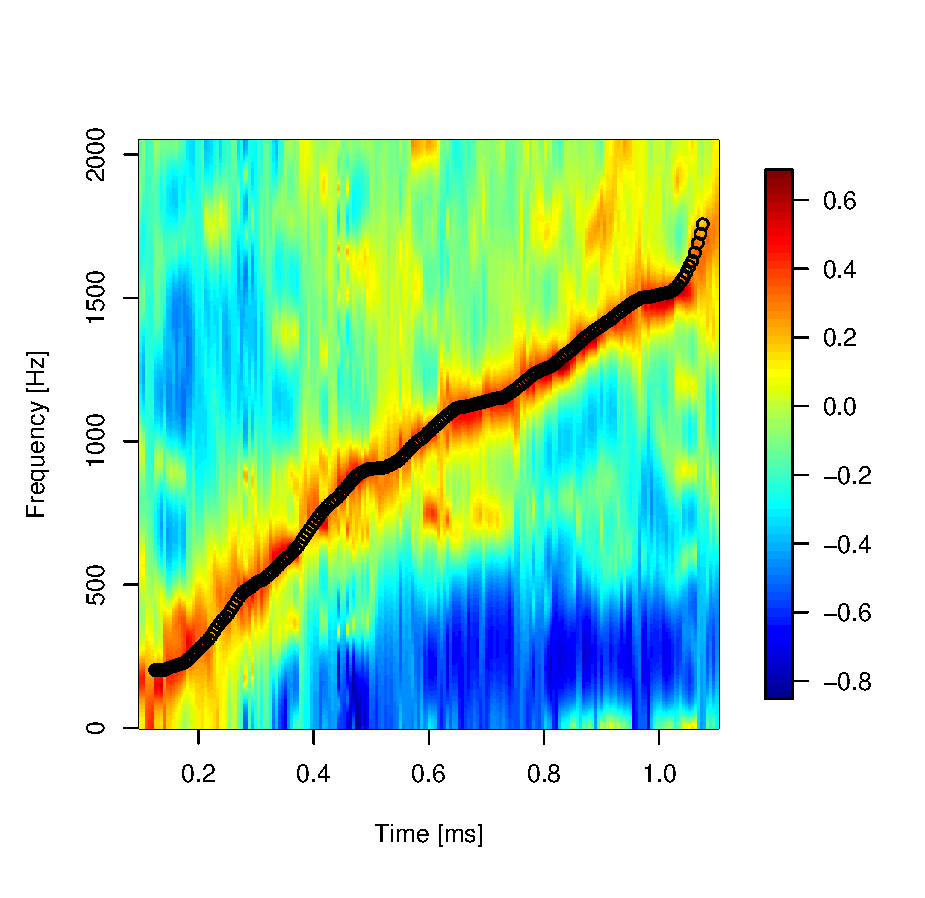
\includegraphics[width=0.5\textwidth]{plots/spectrogram}
 \caption{Spectrogram of the GW signal {\texttt s20S} sampled at \unit[4096]{Hz}.
   The spectrogram is obtained using a data streach of 200 samples overlapping at 90\%
   with each other. The open circles track the ridge $m(t) $ of the $\mbox{}^2 g_2$-mode. } \label{fig:spectrogram}
\end{figure}

We collect the instantaneous frequency $f(t_i)$ corresponding to the ridge $m(t_i)$ for
the midpoint $t_i$ of each local time interval of the spectrogram and interpolate $f(t)$
for values in between $t_i$. We then use our model given by Eq.~\eqref{eq:model1} to obtain
estimates of the time evolution of the ratio together with 95\% confidence intervals.
An example is given in Figure \ref{fig:ratio} where the red triangles are the point estimates and
the grey bands represent 95\% confidence bands. The size of the red triangles is proportional to the magnitude of the $\mbox{}^2 g_2$-mode frequency estimates.
Note that as the frequency of the $\mbox{}^2 g_2$-mode becomes higher our estimates show more uncertainty (bigger intervals) because our model allows for heterogeneous variance. Ratio values
computed using the mass and radius values obtained from the simulation code (i.e.~the true values)
are shown in black. In this example of a noise-free GW signal the coverage of our 95\% confidence band is 100\%
of the true values. In the next section we investigate the performance of the reconstruction of $r(t)$ when the GW
signal is embedded in noise. We also note that despite we have only explicitely shown results for the GW signal of the {\texttt s20S} model the same conclusions hold for any of the other waveforms of our test set.

\begin{figure}
 \centering
 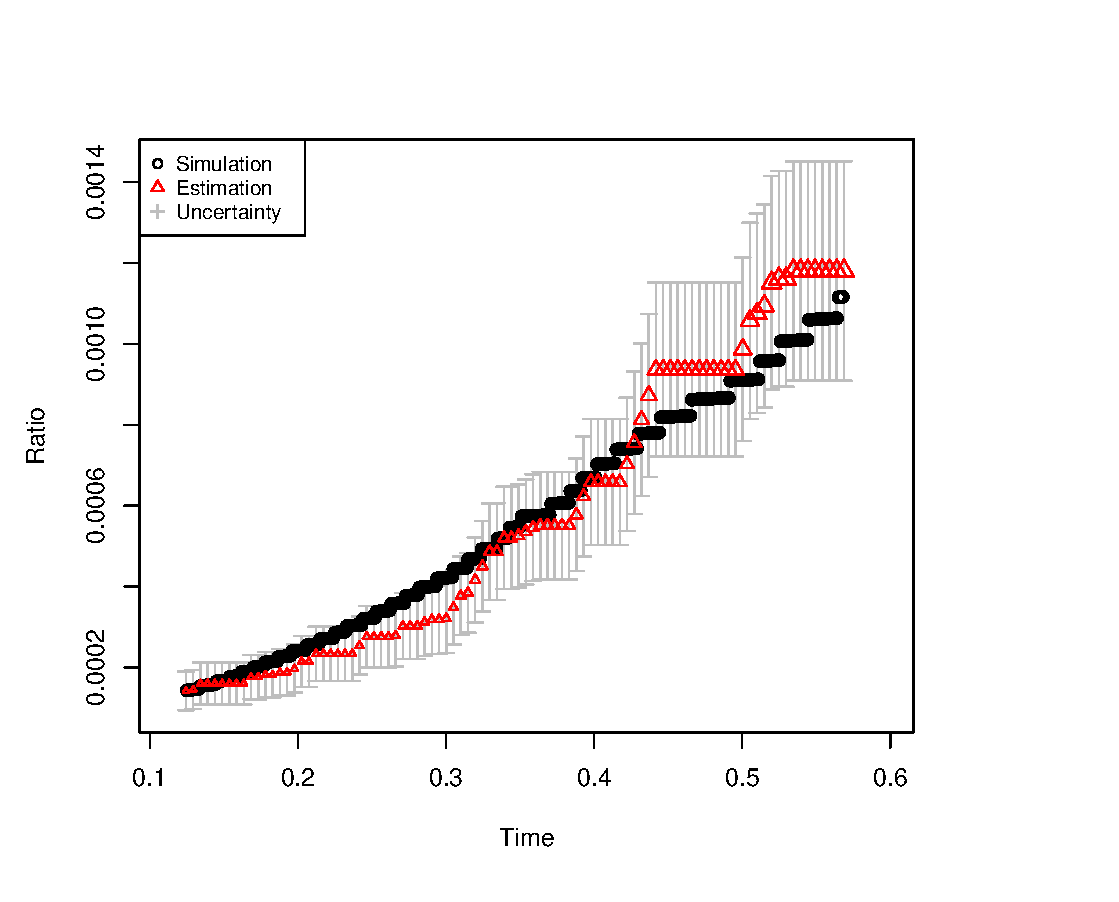
\includegraphics[width=0.5\textwidth]{plots/ratio}
 \caption{Comparison of the time evolution of the ratio $M_{\rm PNS}/R_{\rm PNS}^2$ estimated from the $\mbox{}^2 g_2$-mode of the {\texttt s20S} signal (shown by open triangles and by the 95\% confidence belt in grey) against the value derived from the PNS mass and radius given by the simulation code (shown by filled black circles). The size of the triangles are represented proportionally to the magnitude of the $\mbox{}^2 g_2$-mode frequency estimates.}
 \label{fig:ratio}
\end{figure}


\bigskip

% !TEX root = ccsn.tex
%\section{Detection sensitivity with Advanced gravitational wave detectors}
\section{Detectability prospects}
\label{sec:results}

%\begin{figure}[t]
% \centering
% \includegraphics[width=0.5\textwidth]{plots/spectrum}
% \caption{Amplitude spectral density of the GW detectors aLIGO and AdV at design sensitivity and that of the proposed third-generation detectors Cosmic Explorer and Einstein Telescope. Einstein Telescope sensitivity curve ET-B is obtained pushing second-generation detector technology at its limit. ET-C and ET-D sensitivity curves correspond to a detector configuration where a low-power cryogenic low-frequency interferometer and a high-power room temperature high-frequency interferometer are sharing the same infrastructure~\cite{Hild_2011}. Cosmic Explorer design sensitivity will be achieved in two stages. Stage 1 (CE1) is expected to use the technology developed for the ``A+'' upgrade to aLIGO but scaled up to a 40 km detector while stage 2 (CE2) will implement state-of-the-art technology to decrease quantum and thermal noises~\cite{reitze2019cosmic}.} 
% \label{fig:spectrum}
%\end{figure}

\begin{figure}[t]
  \centering
  \begin{tabular}{c}
    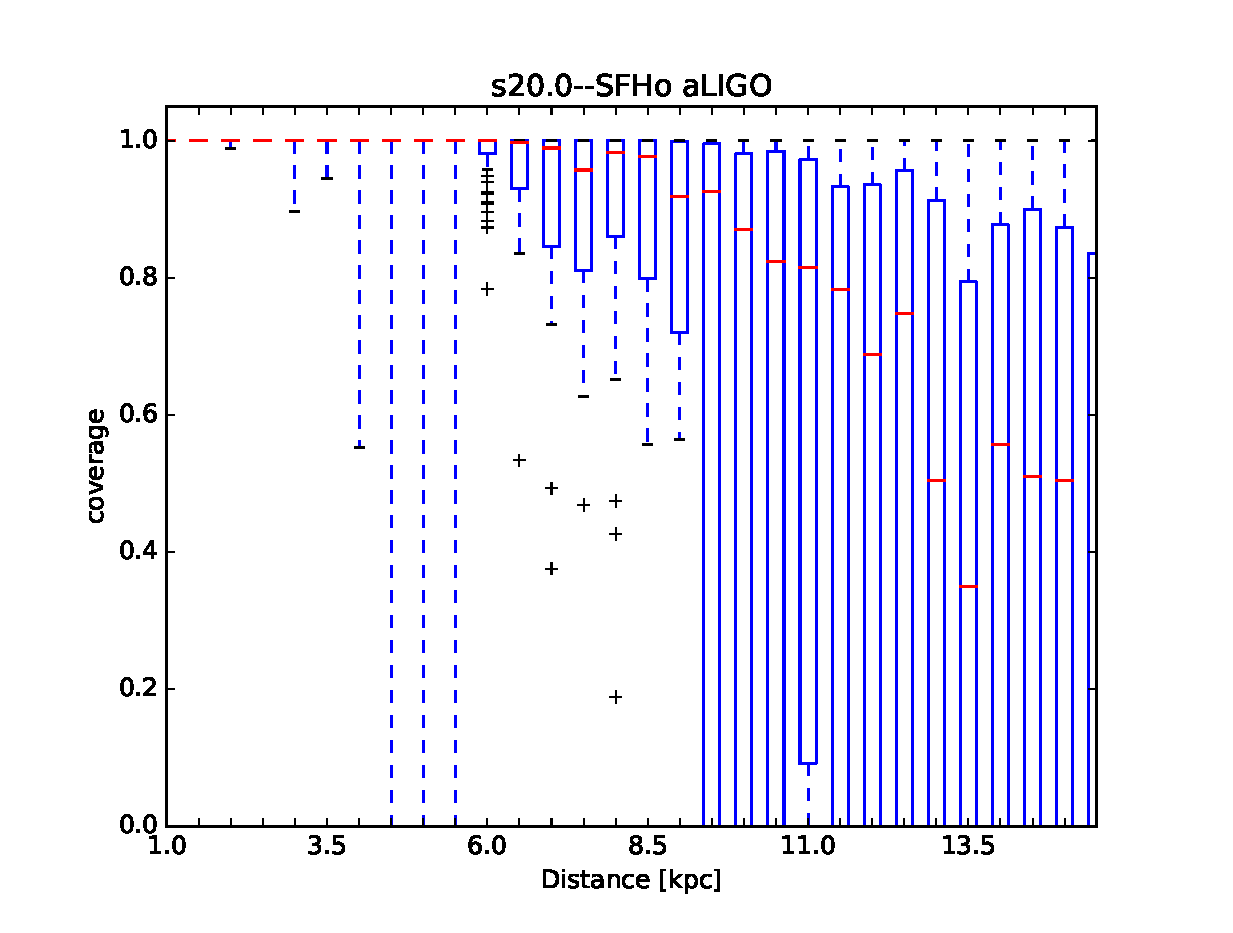
\includegraphics[width=0.5\textwidth]{plots/s20--SFHo_covpbb_boxplot_aLIGO} \\
    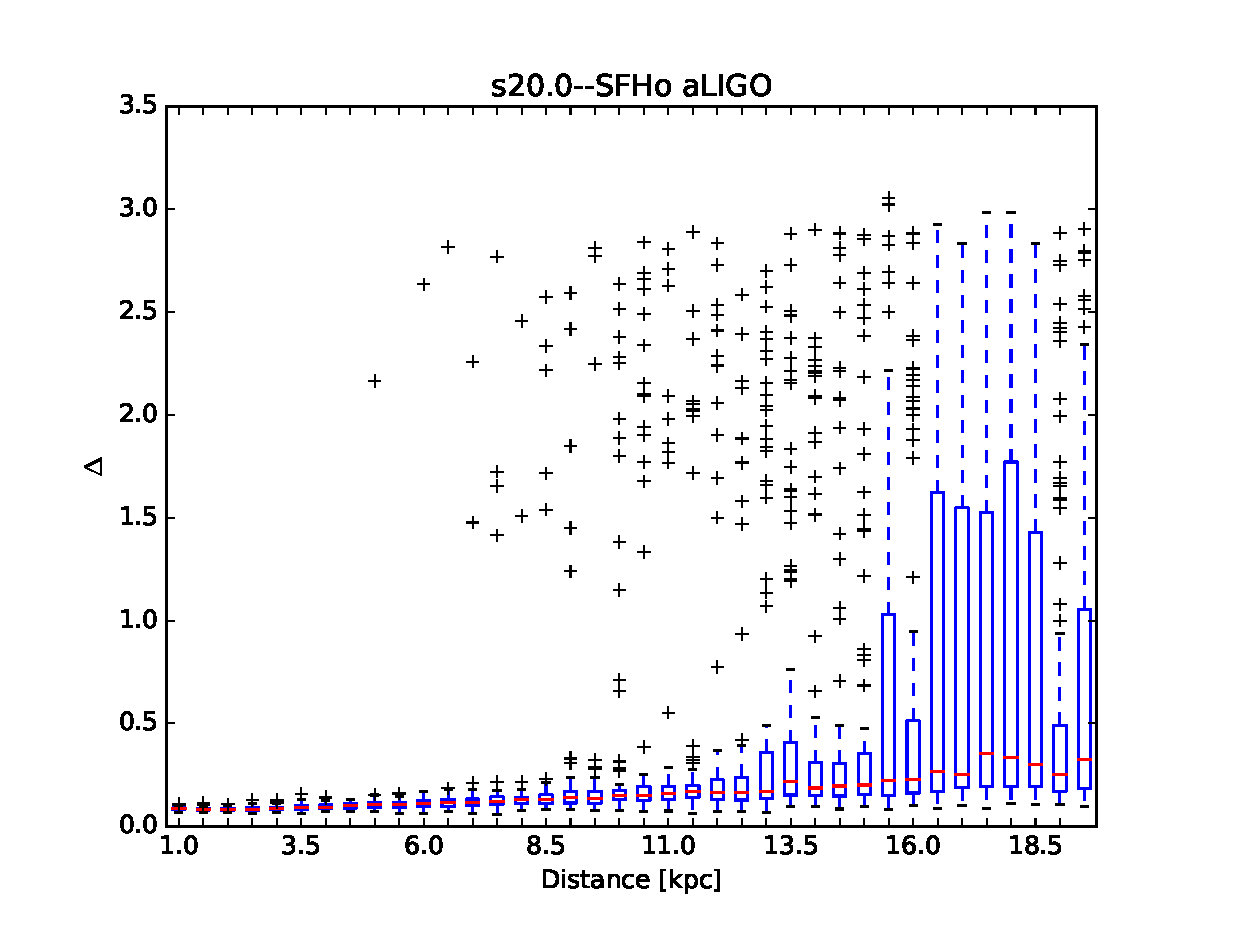
\includegraphics[width=0.5\textwidth]{plots/s20--SFHo_error_boxplot_aLIGO} \\
  \end{tabular}
    
 \caption{Boxplots of the $coverage$ (upper panel) and $\Delta$ (lower panel) for {\texttt s20S} signal embedded in aLIGO noise at different distances from the Earth. 100 noise realizations are considered for each distance. The orange lines indicate the median values while the empty rectangles indicate the first and third quartiles. The ``+'' markers are outliers outside the first and third quartiles.}
  \label{fig:s20results}
\end{figure}

To estimate how accurately we can infer the time evolution of $r(t)$ in the GW data of a single
detector we inject the GW signal for model {\texttt s20S} into 
100 Gaussian noise realisations whose power spectral density (PSD) follows the aLIGO
spectrum~\cite{aLIGOsens:2018}. %The PSD of aLIGO and AdV at design sensitivities, along with those of planned third-generation detectors, are shown in Figure~\ref{fig:spectrum}. 

We cover a large range of distances for which a CCSN detection in second-generation GW detectors is feasible. We assume that the source is optimally oriented with respect to our single detector. Moreover, we also assume that a CCSN GW signal has been identified in the data and that the beginning of the signal is known within {$\mathcal O$}(10 ms). The data (signal embedded in noise) are whitened using the function {\tt prewhiten} of the R-package {\tt TSA}. An auto-regressive model with a maximum of maximal 100 coefficients is used.    

For each of the noise realizations we reconstruct the ratio time series {$r_i$} of length $N$ starting from the left side of the spectrogram and constraining the beginning of the track to be smaller than \unit[200]{Hz}. \mab{This value is chosen using the information on the initial mode frequency from the simulations.}
The reconstructed ratio is then compared to the ``true'' ratio {$r_i^0$} derived from the PNS mass and radius computed from the {\texttt s20S} simulation. The top panel of Fig.~\ref{fig:s20results} shows the distribution of the fraction of the ratio values {$r_i^0$} that fall within the 95\% confidence interval of {$r_i$} as a function of the distance to the source. This quantity, hence, gives information about the {\it coverage} of the reconstructed ratio. The coverage takes maximum values when the source is located within a few kpc and then decreases with the distance.

To better quantify how well we reconstruct the ratio we also consider  the mean of the relative error of $r_i$ along 
the track of the spectrogram, $\Delta$,  
\begin{equation}
\Delta=\frac{1}{N}\sum_1^N\frac{|r_i-r_i^0|}{r_i^0}\,.
\end{equation}
The values of $\Delta$ for each of the 100 noise realizations are shown as a function of the distance
in the bottom panel of Fig.~\ref{fig:s20results}. For a source located up to $\sim$\unit[9]{kpc} the relative error
remains smaller than 20\%. At closer distances $\Delta$ is smaller but it does not vanish. This reflects the approximate nature of the model used for $r$. It is nevertheless remarkable that, on average, one can reconstruct the ratio time series with a good
precision up to distances of $\sim$ 9 kpc (for this particular waveform) with a coverage value
larger than 80\%. We note that there are a few noise realizations for distances below 9 kpc for which
$\Delta$ takes large values, indicating that the method fails to accurately reconstruct the ratio in those cases. \mab{The main cause of failure is the split of the ridge in few blobs when the signal becomes weaker and weaker.}
%\tf{Do we know why that is the case? What is intrinsically different from one noise realisation to another that makes the method more prone to failure? I think we should provide some explanation here, if we have it.}

\begin{figure}[t]
  \centering
  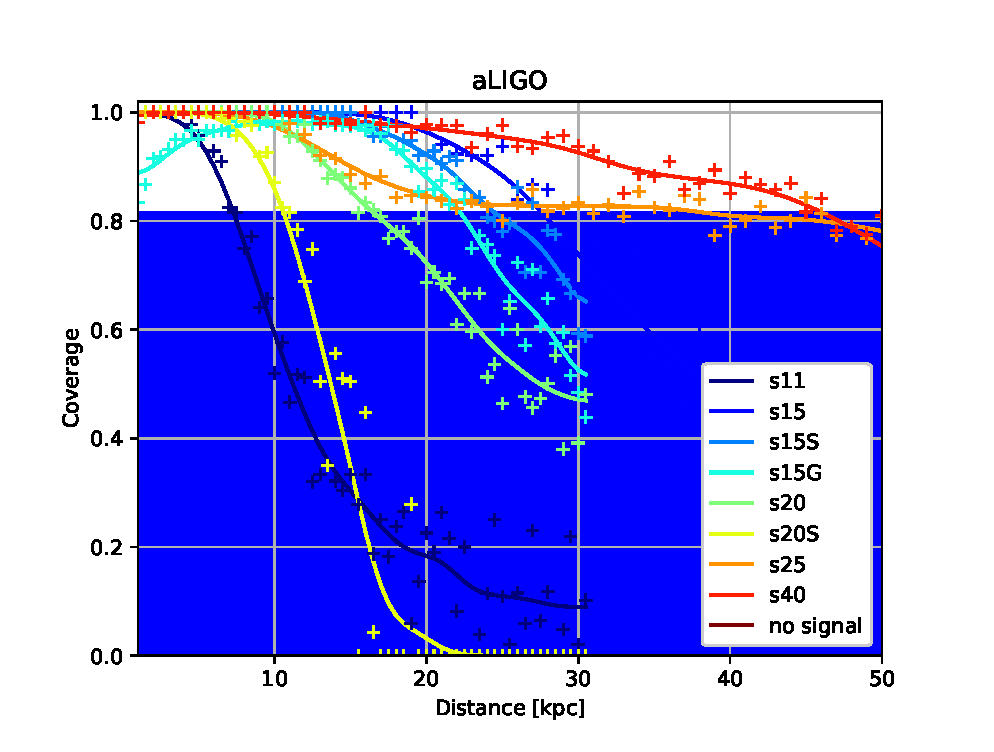
\includegraphics[width=0.5\textwidth]{plots/aLIGO_coverage_allwvfs}
 \caption{Median of the coverage for the eight CCSN waveforms of the {\it test set} embedded in aLIGO noise as a function of the  distance to the source. \mab{The ``no signal'' line shows the median of coverage in absence of any signal. In this example, the median is null and overlaps with the horizontal axis. The blue band boundaries are given by the $\mathrm{5^{th}}$ and $\mathrm{95^{th}}$ percentiles of coverage in absence of any signal.}} \label{fig:aLIGO_cov_allwvf}
\end{figure}

\begin{figure}[t]
  \centering
  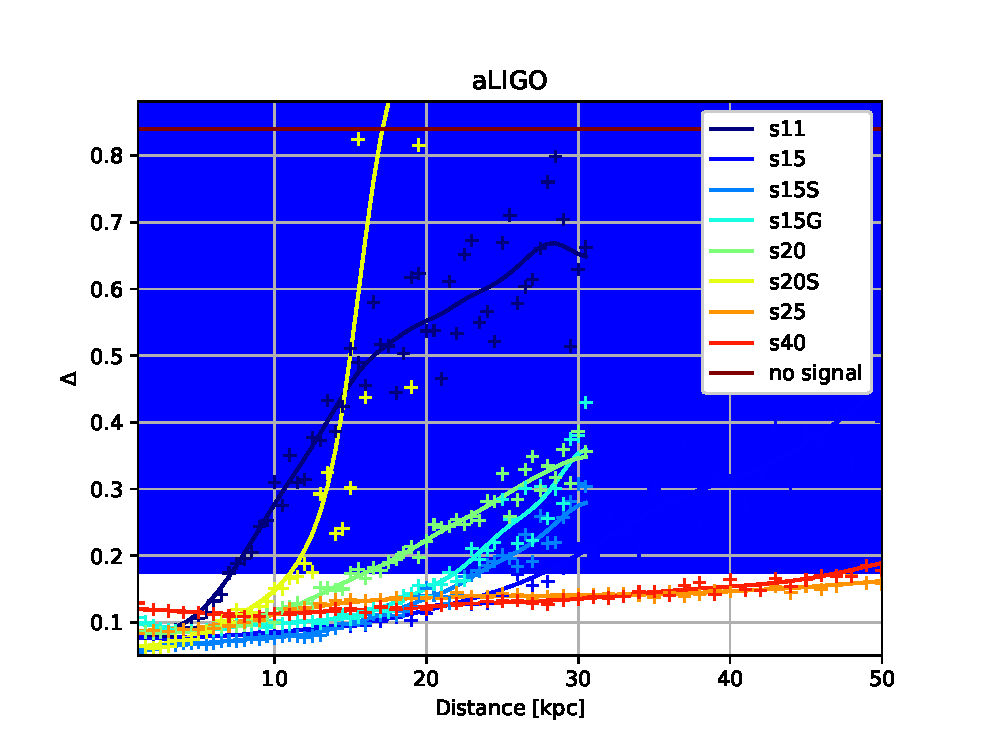
\includegraphics[width=0.5\textwidth]{plots/aLIGO_delta_allwvfs}
 \caption{Same as Fig.~\ref{fig:aLIGO_cov_allwvf} but for the relative error $\Delta$.}
% Median of $\Delta$ for 8 CCSN waveforms embedded in aLIGO noise and located at different distance from the Earth. The ``no signal'' line and band show the median and first and third quartile of $\Delta$ in absence of any signal.} 
\label{fig:aLIGO_prec_allwvf}
\end{figure}

We have tested that the method does not depend on the specific features of the waveform of model {\texttt s20S} by repeating the procedure for the remaining seven waveforms of the {\it test set} described in Section \ref{sec:simulations} covering
a large range of progenitor masses. Figure \ref{fig:aLIGO_cov_allwvf} shows that apart from model {\texttt s11} and to a lesser extent model {\texttt s20S}, the ratio is well reconstructed for all waveforms up to a distance of $\sim$ 15kpc. In an
effort to better determine the maximal distance of the source at which we can reconstruct the ratio we have run 100 simulations without injecting a signal and have measured the corresponding coverage for the reconstructed ratios.
\mab{The median of the coverage as well as the band defined by the $\mathrm{5^{th}}$ and $\mathrm{95^{th}}$ percentiles are shown in Figure \ref{fig:aLIGO_cov_allwvf}.}
The noise only median value is identically zero in this case. However, note that it could be different
from zero because
the g-mode reconstruction algorithm is looking for a continuously  increasing frequency track
in the spectrogram, starting between 0 and 200 Hz, where we expect the GW signal to be.
This is enhancing the probability of overlap. This effect explains why certain values of overlap can reach
values as high as 80\% even when no signal is added to the noise. \tf{I don't understand this last comment.} \mab{Toni: is that clearer?}

Figure \ref{fig:aLIGO_prec_allwvf} shows the relative error $\Delta$ as a function of the distance for the signals of the {\it test set}
as well as the result when only noise is considered. This quantity follows the same trend than that followed by the coverage, since all signals but models {\texttt s11} and {\texttt s20S} are reconstructed with relative errors below 20\% up to distances of $\sim$ 15kpc. Correspondingly, the no-signal case yields the largest error, as expected.

We perform the same analysis using the design sensitivity curve of AdV and expected sensitivity curves for third-generation 
GW detectors. The results for the former are reported in Table \ref{tab:results} and are discussed below. We focus now on third-generation detectors, presenting our findings in Table \ref{tab:results} and in Fig.~\ref{fig:s20--SFHo_all3G}. In Europe the Einstein Telescope project proposes to host in a 10-km equilateral triangle configuration three low-power, low-frequency, cryogenic interferometers as well as three high-power, high-frequency interferometers. Three sensitivity curves, ET-B, ET-C and ET-D corresponding to different options and stages of the project~\cite{Hild_2011} are considered in our study. %(cf.~Fig.~\ref{fig:spectrum}).
The US based project Cosmic Explorer~\cite{reitze2019cosmic} is expecting to reach its design
sensitivity circa 2040 through two phases labeled CE1 and CE2. %Their corresponding sensitivity curves are also shown in Fig.~\ref{fig:spectrum}. 

\begin{figure}[t]
  \centering
  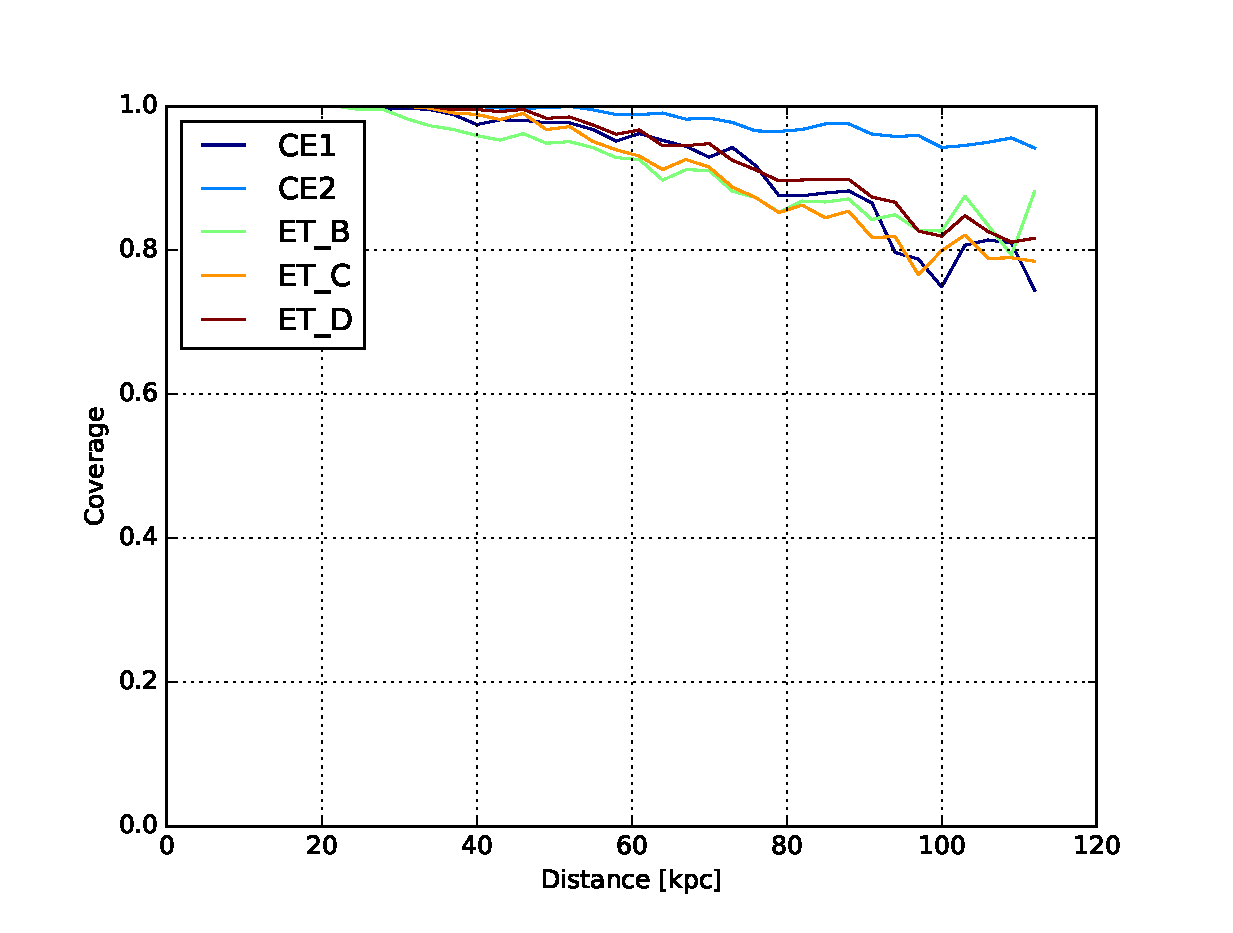
\includegraphics[width=0.5\textwidth]{plots/s20--SFHo_all3G}
  \caption{Median of the relative error $\Delta$ as a function of the  distance to the source for the CCSN waveform model {\texttt s20S} embedded in third-generation detector noise.}
  \label{fig:s20--SFHo_all3G}
\end{figure}

Figure \ref{fig:s20--SFHo_all3G} displays $\Delta$ as a function of the source distance for the five third-generation detector configurations we analyze. As before, we use the {\texttt s20S} waveform model as a reference case.  This figure shows that,  overall, the ratio is well reconstructed up to distances in the range \unit[100--200]{kpc} which represents an order of magnitude improvement with respect to aLIGO and AdV. We also note that the results for the various Einstein Telescope configurations lay in between those of the two Cosmic Explorer designs. Moreover,  the detectability prospects for the former depend weakly on the detector configuration while the arrangement of CE2 yields better results than CE1. These results are confirmed for all other waveforms of our sample except for model {\texttt s25} for which the maximal distance reach in CE2 is significantly lower than CE1, as shown in Fig.~\ref{fig:distances}. This is partly due to the small variation of the reconstruction quality to the distance of the source making the estimation of $d_r$ rather uncertain for this particular waveform. \tf{Is this really understood? What's particular in this waveform?}

\begin{figure}[t]
  \centering
  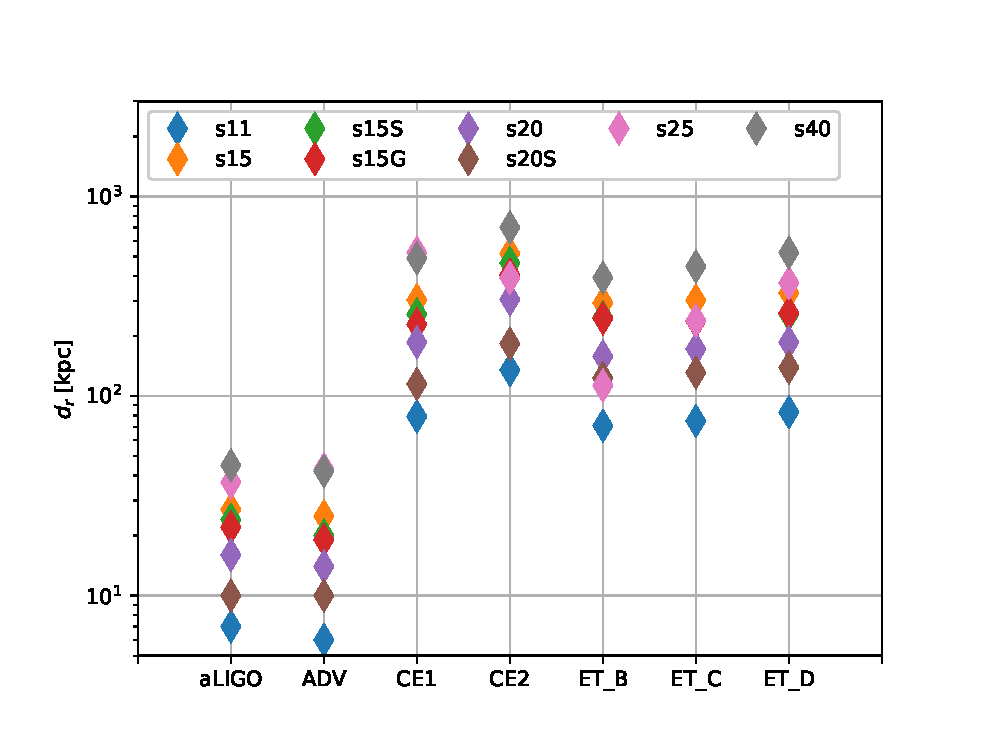
\includegraphics[width=0.5\textwidth]{plots/dist_allwvfs_2G3G}
  \caption{Maximal distance at which the ratio $r=M_{\rm PNS}/R_{\rm PNS}^2$ is reconstructed
    with good accuracy for all GW detectors analyzed in this study. The values are shown for all eight CCSN waveforms of our sample assuming that the source is optimally oriented with respect to the detector. Some waveform maximal distance markers are not visible because the do overlap (for instance \texttt{s15G} is overlapping with \texttt{s25} for CE2).} 
\label{fig:distances}
\end{figure}

\begin{table}
  \centering
  \begin{tabular}{c|c|cccccccc}

\multicolumn{2}{c|}{}  & \texttt{s11} & \texttt{s15} & \texttt{s15S} & \texttt{s15G} & \texttt{s20} & \texttt{s20S} & \texttt{s25}  & \texttt{s40}\\   

\hline
\multirow{3}{*}{aLIGO} & $d_{r}$   & 7 & 28 & 24  & 22 & 16 & 11 & 38 & 46 \\
\cline{2-10}
                       & $d_{\rm det}$ & 11 & 36 & 26 & 27 & 21 & 16 & 74 & 61\\
%                      & SNR      & 14 & 46 & 33 & 35 & 27 & 21 & 96 & 80\\

\hline
\hline
\multirow{3}{*}{AdV}   & $d_{r}$   & 7  & 26  & 20 & 19 & 15 & 10 & 43 & 42 \\
\cline{2-10}
                       & $d_{\rm det}$ &  10 & 32 & 22 & 23 & 18 & 13 & 64 & 52\\
%                      & SNR      &  13 & 41 & 29 & 30 & 23 & 17 &  83 & 68\\

\hline
\hline
\multirow{2}{*}{CE1}   & $d_{r}$   & 79  & 304 & 258 & 229 & 187 & 115 & 524 & 490 \\
\cline{2-10}
                       & $d_{\rm det}$ & 115 & 377 & 270 & 282 & 217 & 168 & 774  & 633\\
%                      & SNR      & 149 & 490 & 352 & 366 & 282 & 218 & 1006 & 822\\

\hline
\multirow{2}{*}{CE2}   & $d_{r}$  & 135 & 499 & 451 & 405 & 305 & 183 & 391 & 898 \\
\cline{2-10}
                       & $d_{\rm det}$ & 197 & 649 & 468 & 489 & 375 & 294 & 1347  & 1100\\
%                      & SNR    & 256 & 843 & 608 & 635 & 487 & 382 & 1751 & 1430\\

\hline
\multirow{2}{*}{ET\_B} & $d_{r}$ & 71  & 293 & 248 & 245 & 158 & 123 & 113 & 392 \\
\cline{2-10}
                       & $d_{\rm det}$ & 106 & 364 & 274 & 391 & 216 & 200 & 805 & 665\\
%                      & SNR      & 138 & 473 & 356 & 379 & 381 & 260 & 1046 & 865\\

\hline
\multirow{2}{*}{ET\_C} & $d_{r}$ & 75  & 302 & 239 & 237 & 172 & 131 & 239 & 446 \\
\cline{2-10}
                       & $d_{\rm det}$ & 97 & 332 & 246 & 260 & 194 & 164 & 727  & 603\\
%                      & SNR      & 126 & 432 & 320 & 338 & 252 & 213 & 945 & 783\\

\hline
\multirow{2}{*}{ET\_D} & $d_{r}$ & 83  & 329 & 257 & 261 & 186 & 139 & 369 & 523 \\
\cline{2-10}
                       & $d_{\rm det}$ & 107 & 368 & 271 & 285 & 213 & 174 & 796  & 661\\
%                      & SNR      & 140 & 477 & 352 & 371 & 277 & 227 & 1034 & 859 \\

  \end{tabular}
  \caption{%%
  Maximal distance $d_{r}$ at which the ratio $r=M_{\rm PNS}/R_{\rm PNS}^2$ is reconstructed
    with good accuracy for all GW detectors analyzed in this study, assuming optimal orientation between the source and the detector. Correspondingly, $d_{\rm det}$ is the distance at which different interferometers could detect a source
    optimally oriented with a matched filter signal-to-noise ratio of 13. All distances are expressed in kpc.
    %%
  }
  \label{tab:results}
\end{table}

All results for both second-generation and third-generation detectors are summarized in Table \ref{tab:results} and Figure
\ref{fig:distances}. Table \ref{tab:results} reports the source distances $d_r$ in kpc at which the median of the coverage is lower than 95\% of the noise only values for aLIGO, AdV, and different configurations of third-generation detectors. This same information is displayed in Fig.~\ref{fig:distances}. We have checked that using either the median of the coverage or the median of $\Delta$ yields similar results for the distance. On the other hand, the quality of the ratio reconstruction and, thus, of the distance range, depends on the signal-to-noise ratio, expressed in Table \ref{tab:results} by $d_{\rm det}$. The numbers reported on the table for $d_r$ are an estimate of the order of magnitude of the maximal distance of the source  at which a
reconstruction of the ratio could be possible with current and planned GW detectors. We also provide upper limits for $d_{\rm det}$ by taking into account the detector antenna response in our simulations and assuming that the source is optimally oriented with a matched filter signal-to-noise ratio of 13. Table \ref{tab:results} shows that the results for the Advanced Virgo detector at design sensitivity are very similar to those of aLIGO, despite the differences in detector sensitivity. It is remarkable that for third-generation detectors the PNS surface gravity  could be reconstructed for sources located up to a few hundreds of kpc. It is nevertheless important to note the rather wide range in distances we obtain for the different waveforms of our {\it test set} that probe a large range of progenitor masses. We do not find any correlation between either the mass of the progenitor nor the EOS with $d_r$.

\bigskip

\section{Conclusion}
The algorithm presented in this paper is a first attempt to infer the time evolution of a
combinaison of the mass of the PNS and its radius based on the universal relations found
in PNS asteroseismology. More precisely, we have considered in this paper the ratio
$r=M_{\rm PNS}/R_{\rm PNS}^2$ derived from the observation of the $\mbox{}^2g_2$
oscillation mode in the GW data. We have especially investigated the performance of the algorithm
in the case of an optimally oriented source detected in a singe GW detector. For Advanced LIGO
or Advanced Virgo, the ratio can be reconstructed for a source in the Galaxy. We have shown
that this is true for a wide range of progenitor masses and that the quality of the inference
mainly depends on the signal-to-noise ratio of the signal. For third generation of GW detectors such
as Einstein Telescope and Cosmic Explorer, the $\mbox{}^2g_2$ will be reconstructible for sources
at distances of several kpc. Cosmic Explorer in its stage 2 configuration is obtaining the best performance
for all waveforms considered here thanks to its excellent sensitivity in the \unit[100-1000]{Hz} range.
Among the three configuration of Einstein Telescope, ET-D is providing the best performance,
especially for the waveforms with the highest progenitor mass (25 $\Msol$ and 40 $\Msol$). Comparing
$d_r$ for ET-B and the other third generations projects, it seems that having a good sensitivity
below \unit{200}[Hz] is important for massive mass progenitor signals.

%The model to infer the ratio as function of the frequency is based on 1D {\sc AENUS-ALCAR} simulations.
%We have observed that using the other numerical code {\sc CoCoNut} inputs lead to systematic bias of the
%ratio reconstruction. 

This study does not include the realistic case of operating within a network of detectors. We defer this
for a forthcoming publication. The sources of GWs we have considered here are optimally oriented. The
reported distance at which we can infer the time evolution of $r=M_{\rm PNS}/R_{\rm PNS}^2$ are thus an
upper limit that may be lower by a factor 2--3 on average for a source located anywhere on the sky.

Finally, this method can be adapted to other PNS oscillation modes, changing few parameters such as
the frequency range of the beginning of the mode and its monotonic raise or descent. Being able to
reconstruct several modes in the same GW signal would allow to infer individually each of the PNS property.

\bigskip


\bigskip\noindent\textit{Acknowledgments} ---

\begin{appendices}
\section{G-mode reconstruction}
\label{app:gmode}
Given the spectrogram and an specified time interval for the g-mode reconstruction, our proposal method works as follows.  The starting point must be specified.  It can be either at the beginning or at the end of the signal.  Then, in one of these extremes, the maximum energy value is identified, registering its frequency.  This is done independently for a number of consecutive time intervals.  Then we calculate the median of these frequency values, providing a robust starting value for the g-mode reconstruction.

The starting frequency value is the first g-mode estimate for the first or the last time interval, depending on the specified starting location.  If the reconstruction is set to start at the beginning of the signal, the reconstruction will be done progressively over the time intervals, where each maximum frequency value will be calculated within a frequency range specified by the previous g-mode estimate.  Given the non-decreasing behaviour of the true g-mode values, the g-mode estimates will be forced to be greater or equal than the one estimated for its previous time interval, and lower than a specified upper limit.  As a result, the g-modes estimates will be a non-decreasing sequence of frequency values. 

If the reconstruction is set to start at the end of the signal, the g-modes will be estimated backward in time.  Each maximum frequency is calculated within a range determined by its successor (in time) g-mode estimate.  These estimates are forced to be lower or equal than its successor (in time) estimate, but greater than a specified lower limit. Thus, a non-decreasing sequence of g-mode estimates is guaranteed.

This g-mode reconstruction method works if and only if the signal is strong enough to provide information about the g-mode, which is reflected in the spectrogram.


Given the sequence of g-mode estimates, the confidence band will be calculated by using the model defined in \eqref{eq:model1}. The g-mode estimates are frequency values which we use as predictors in the model in order to generate confidence intervals for the ratios. Since the g-mode estimates are indexed by time, the confidence intervals for the ratios are too.  Thus, we generate the confidence band by interpolating the lower and upper limits of the collection of consecutive confidence intervals, which will be valid for the time range of the g-mode estimates.  This confidence band is used to estimate the coverage probabilities in our simulation studies presented \pcd{\sout{below} above}.  

\end{appendices}
%\bibliographystyle{unsrt}
\bibliography{biblio}


\end{document}
